% from Andrew Blanks
\documentclass[11pt,a4]{article}
\usepackage[top=0.85in,left=1in,footskip=0.75in,marginparwidth=2in]{geometry}

% use Unicode characters - try changing the option if you run into troubles with special characters (e.g. umlauts)
\usepackage[utf8]{inputenc}

% clean citations
\usepackage{cite}
\usepackage{mathtools}
% hyperref makes references clicky. use \url{www.example.com} or \href{www.example.com}{description} to add a clicky url
\usepackage{nameref,hyperref}
\usepackage{enumerate}
% line numbers
\usepackage[right]{lineno}

% improves typesetting in LaTeX
\usepackage{microtype}
\DisableLigatures[f]{encoding = *, family = * }

% text layout - change as needed
\raggedright
\setlength{\parindent}{0.5cm}
\textwidth 6.25in 
\textheight 8.75in

% use adjustwidth environment to exceed text width (see examples in text)
\usepackage{changepage}

% adjust caption style
\usepackage[aboveskip=1pt,labelfont=bf,labelsep=period,singlelinecheck=off]{caption}

% remove brackets from references
\makeatletter
\renewcommand{\@biblabel}[1]{\quad#1.}
\makeatother

% headrule, footrule and page numbers
\usepackage{lastpage,fancyhdr,graphicx}
\usepackage{epstopdf}
\pagestyle{myheadings}
\pagestyle{fancy}
\fancyhf{}
\rfoot{\thepage/\pageref{LastPage}}
\renewcommand{\footrule}{\hrule height 2pt \vspace{2mm}}
\fancyheadoffset[L]{2.25in}
\fancyfootoffset[L]{2.25in}

% use \textcolor{color}{text} for colored text (e.g. highlight to-do areas)
\usepackage{color}

% define custom colors (this one is for figure captions)
\definecolor{Gray}{gray}{.25}

% this is required to include graphics
\usepackage{graphicx}

% use if you want to put caption to the side of the figure - see example in text
\usepackage{sidecap}

% use for have text wrap around figures
\usepackage{wrapfig}
\usepackage[pscoord]{eso-pic}
\usepackage[fulladjust]{marginnote}
\reversemarginpar

\usepackage{float}
% document begins here
\begin{document}
\vspace*{0.35in}

% title goes here:
\begin{center}
{\Huge
\textbf
\newline{Title-Here}
}
\newline
\newline

% authors go here:
\Large
Joe Blogs\textsuperscript{1§},
Jane Blogs\textsuperscript{1§},

\end{center}

\begin{flushleft}
\bigskip
{1.} Address goes here\\
\bigskip
*Corresponding author E-mail: \\
§Joint first author
\end{flushleft}
\newpage
\section*{Abstract}
\begin{justify}
Abstract text goes here
\end{justify}

% now start line numbers
\linenumbers

% the * after section prevents numbering
\section*{Introduction}
\begin{justify}
Introduction text goes here

\end{justify}

\section*{Materials and Methods}

\subsection*{Materials} 
 Materials text goes here
 
\subsection*{Method1}  
Method 1 text goes here

\subsection*{Method2}
Method 2 text goes here

\subsection*{Data analysis}
Data analysis section goes here




% figure goes here but can be moved to wherever it looks best
\begin{figure}
     \centering
     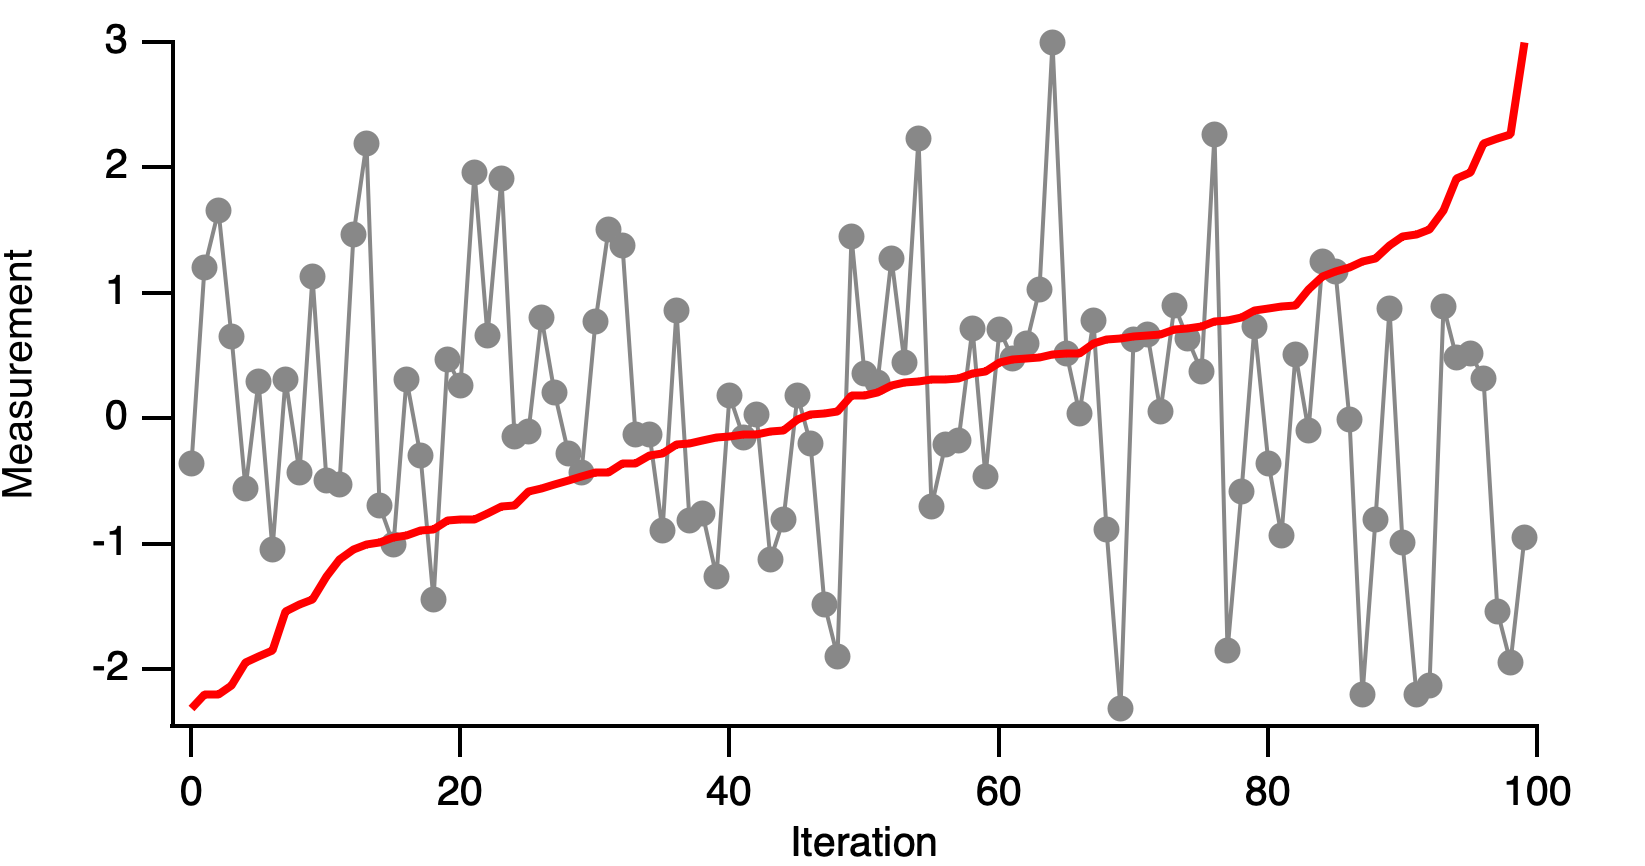
\includegraphics[width=10cm]{Fig_1}
        \caption{
                \textbf{A}:~Blah
                \textbf{B}:~Blah
                \textbf{C}:~Blah
                \textbf{D}:~Blah
        }
        \label{fig:1}
\end{figure}

\section*{Results}
\begin{justify}
Results text goes here 
% reference figure 1 by
(Fig.~\ref{fig:1}).
\subsection*{Blah}
Subsection of results Blah goes here
\end{justify}

\section*{Discussion}
\begin{justify}
Text of discussion goes here
\end{justify}


\section*{Conclusion}
\begin{justify}
Conclusion text goes here

\end{justify}

\section*{Acknowledgments}

Acknowledgments go here

\nolinenumbers

%This is where your bibliography is generated. Make sure that your .bib file is actually called library.bib
\bibliography{Blah}

%This defines the bibliographies style. Search online for a list of available styles.
\bibliographystyle{abbrv}

\end{document}